% ======================================================================
% Paket E: 7.4.2 Kollisionsmodell, 7.4.3 Bahnplaner, 7.4.4 Laufzeitüberwachung
% Entwurf 27.11.2026 für Kapitel/07_Umsetzung.tex (nach \subsection{Regelkette und inverse Kinematik} einfügen).
% Code-Bezug: Repo NilsMeier1812/G1, PR #62 (noch nicht gemergt) @e452513 = BA-Stable 6a40e47 + 2 Commits
% (geändert nur arm_planner.py, arm_planner_process.py, arm_geometry.py). Pfade relativ zur Repo-Wurzel.
% Stellen, die erst mit PR #62 gelten, tragen \pruefen{Stand PR \#62 ...}.
% Zahlen der Planer-Studie vom 26.11. stehen bewusst NICHT hier (gehören in die Evaluation).
% ======================================================================

\subsection{Kollisionsmodell}
\label{sec:kollisionsmodell}

% Rückbezug tab:schutzmechanismen (Vermeiden: Kollisionsprüfung und geplante Bahnen), Hüllkörper sec:kollision_sdt.
Bahnplaner und Laufzeitüberwachung rechnen mit einem Kugelmodell der Arme und Hände, weil beide Abstände für viele Armstellungen in kurzer Zeit brauchen.
Das Modell setzt die Kollisionsprüfung aus Tabelle~\ref{tab:schutzmechanismen} mit dem Hüllkörper um, dessen Schnitttest nach Abschnitt~\ref{sec:kollision_sdt} am einfachsten ist.
% DB: g1pilot/g1pilot/manipulation/arm_geometry.py:3-31 @e452513

% Erzeugung und Auflösung der Kugelsätze.
Das Kugelmodell entsteht beim Start selbsttätig aus den Kollisionsnetzen des Robotermodells.
Ein Clusterverfahren teilt die mit höchstens 5\,mm Punktabstand abgetastete Oberfläche jedes Kettenglieds in Gruppen und legt um jede Gruppe eine Kugel, die alle ihre Punkte einschließt.
Gegen die Umgebung gelten Radien bis 2,2\,cm an der Hand und bis 4\,cm am übrigen Arm.
Gegen den eigenen Körper und den anderen Arm genügen Kugeln bis 5\,cm ab dem Ellbogen, und der Körper selbst ist mit Kugeln bis 9\,cm angenähert.
Abbildung~\ref{fig:kugelmodell} zeigt den Kugelsatz der Hand, der für eine ausgetauschte Hand auf dieselbe Weise entsteht (Abschnitt~\ref{sec:hand_profile}).
% DB: g1pilot/g1pilot/manipulation/arm_geometry.py:39-62,114-149,195-250,335-436 @e452513, Daten/kugelmodell/README.md (Abbildung aus Stand fdb9cba, arm_geometry.py bis 6a40e47 unverändert)

\begin{figure}[htbp]
  \centering
  % Kugelmodell des Armplaners als 3D-Ansicht (orthografisch), linke Hand, gleicher Maßstab in a) und b).
% Eigene Darstellung, Renderings aus dem G1-Code (siehe Daten/kugelmodell/README.md).
\begin{tikzpicture}[ba]
  \node[anchor=north west, inner sep=0] (A) at (0,0) {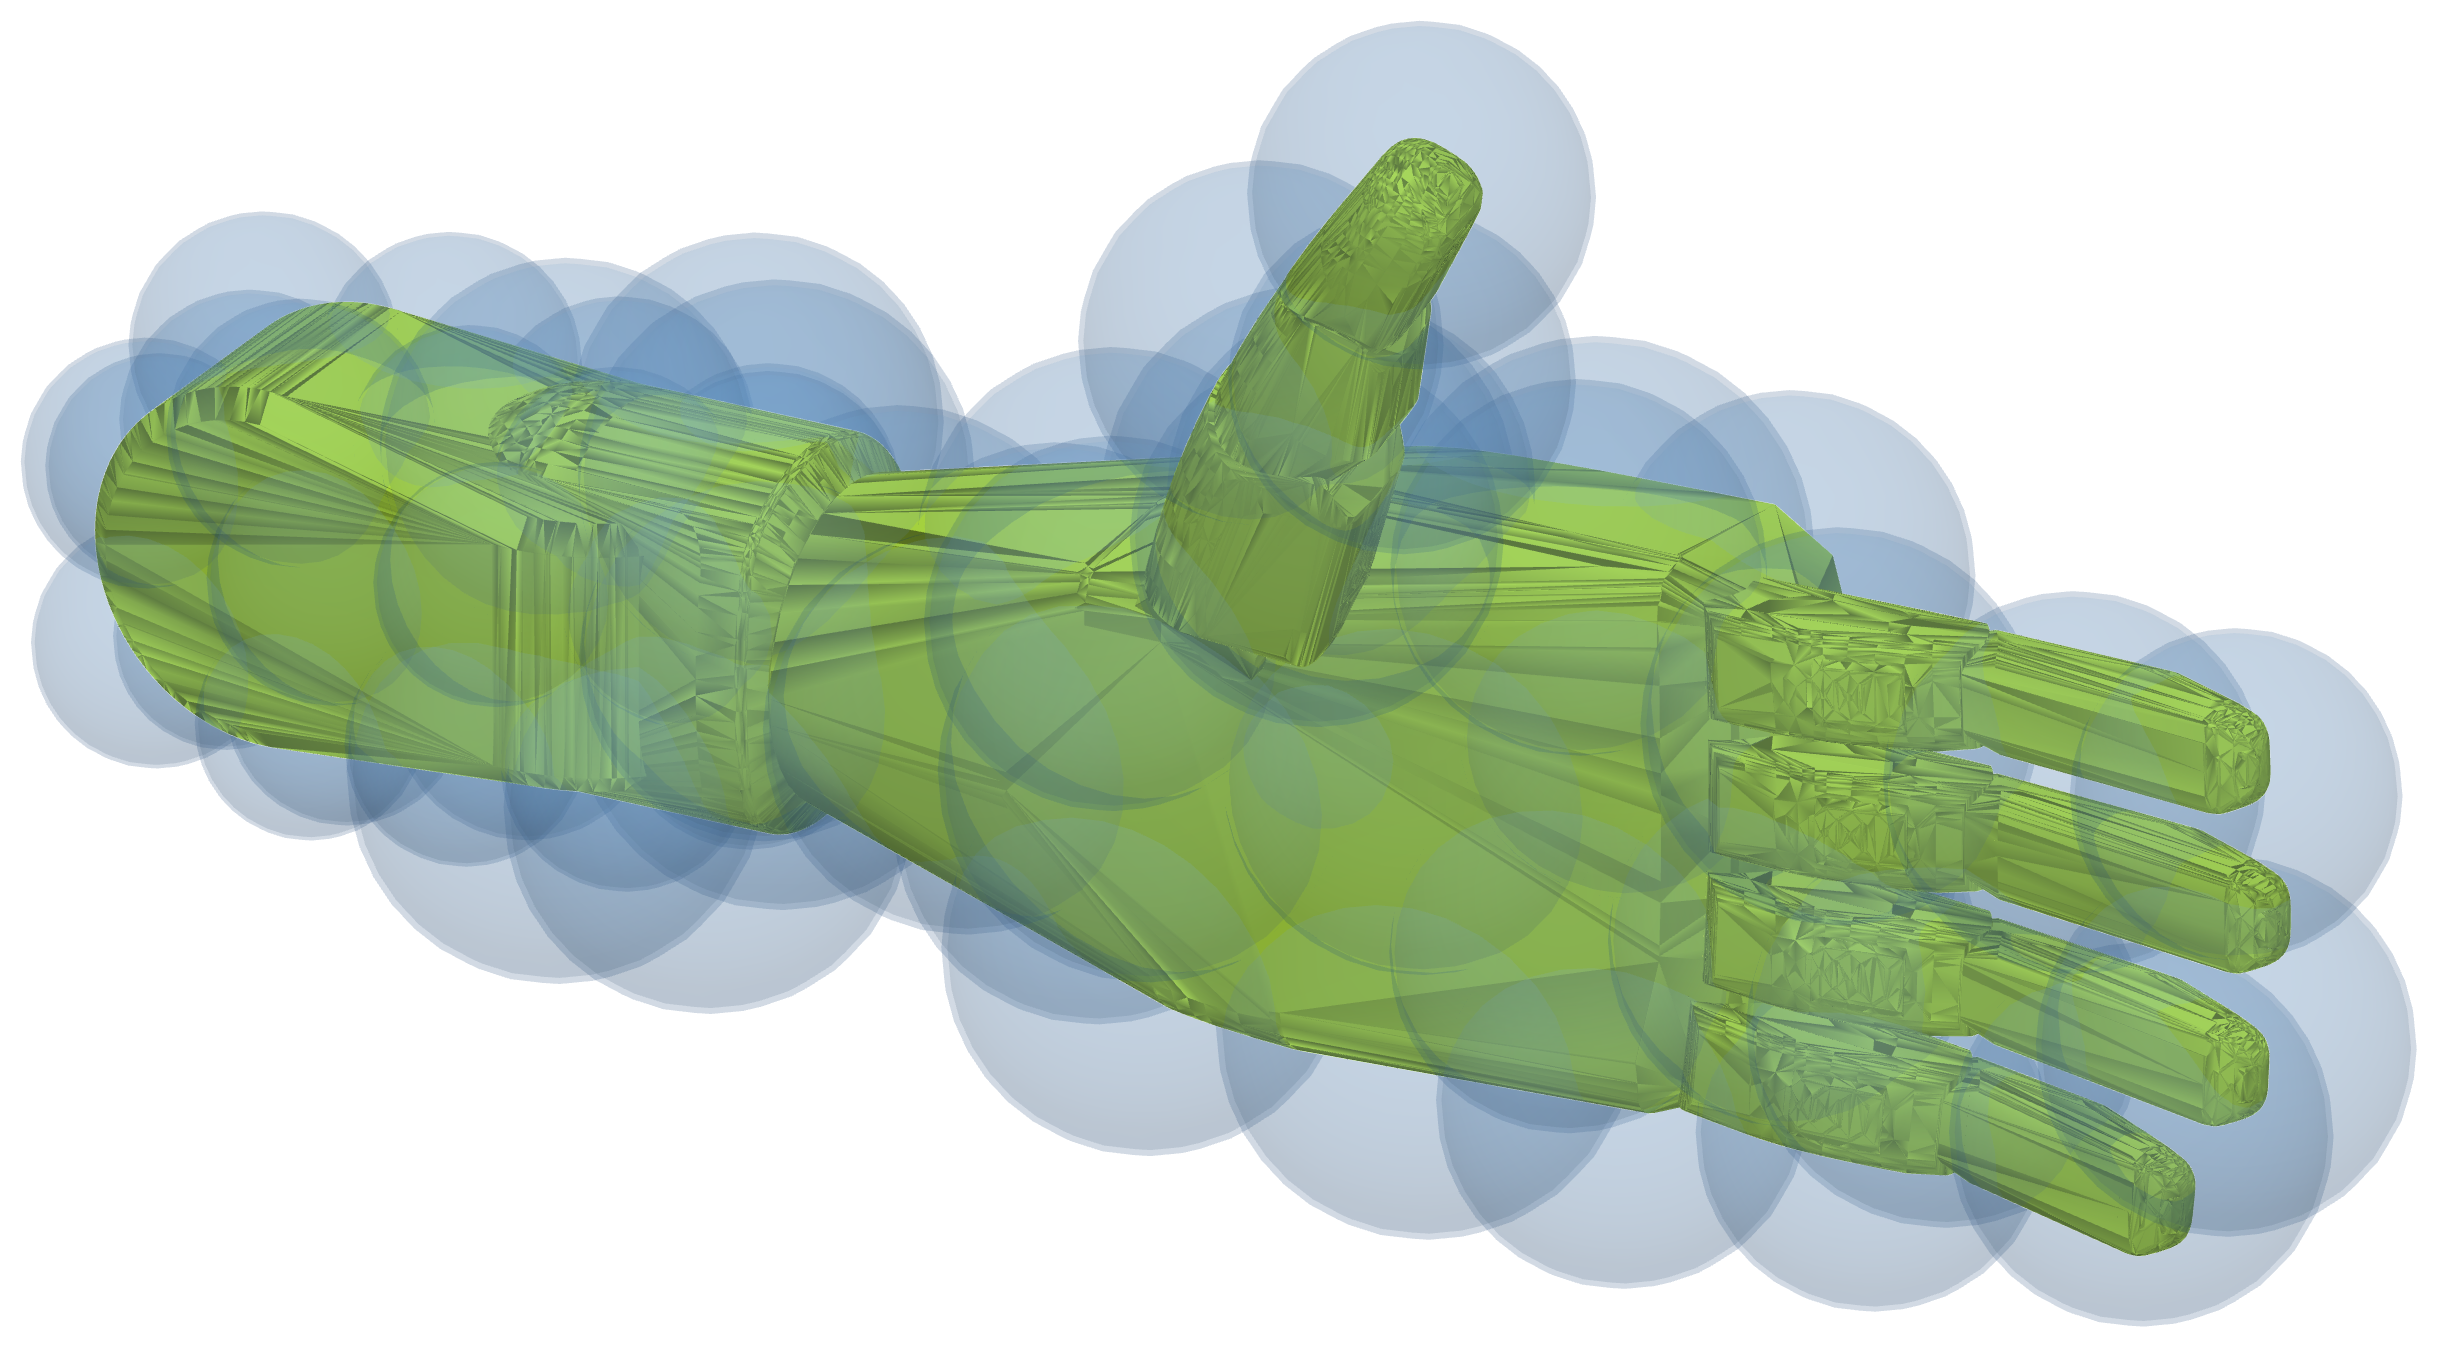
\includegraphics[width=14cm]{Bilder/kugelmodell-3d-inspire.png}};
  \node[ba teiltitel, anchor=north west] at ($(A.south west)+(0,-0.1)$) {a) Inspire-Hand (Modell auch für die Rubber Hand verwendet)};
  \node[anchor=north west, inner sep=0] (B) at ($(A.south west)+(0,-0.9)$) {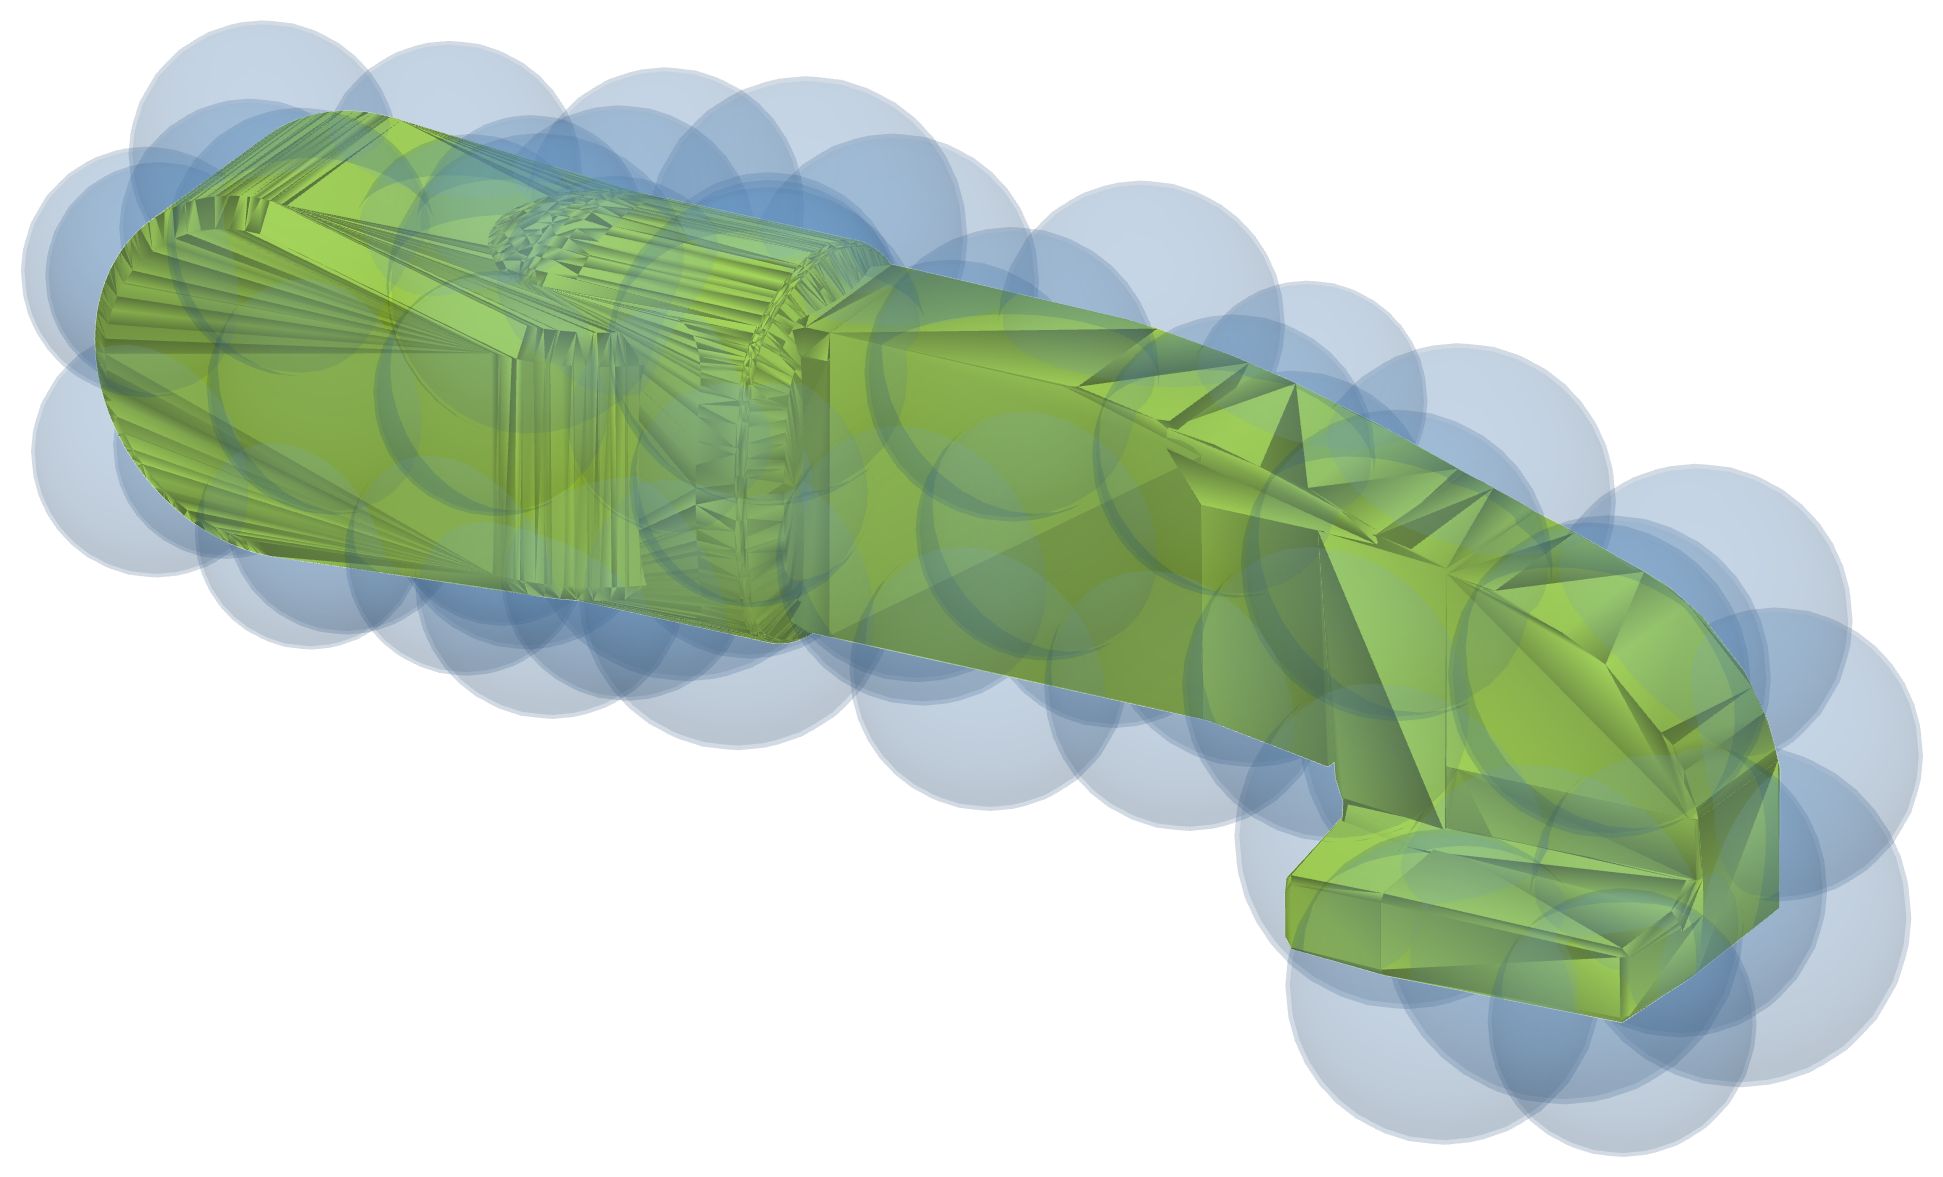
\includegraphics[width=11.16cm]{Bilder/kugelmodell-3d-haken.png}};
  \node[ba teiltitel, anchor=north west] at ($(B.south west)+(0,-0.1)$) {b) Gedruckter Box-Haken (Hand-Profil)};
  \fill[baGruen, draw=baGruen] ($(B.south west)+(0,-1.0)$) rectangle ++(0.4,0.3);
  \node[anchor=west] at ($(B.south west)+(0.45,-0.85)$) {Kollisionsgeometrie};
  \fill[baHellblau, fill opacity=0.45, draw=baBlau, draw opacity=0.5] ($(B.south west)+(4.4,-0.85)$) circle (0.17);
  \node[anchor=west] at ($(B.south west)+(4.65,-0.85)$) {Kugel des Planers};
\end{tikzpicture}

  \caption[Kugelmodell der Hand]{Kugelsatz der linken Hand für die Prüfung gegen die Umgebung. Die Kugeln umschließen die Kollisionsgeometrie der Hand und ragen deshalb über ihre Oberfläche hinaus.}
  \label{fig:kugelmodell}
\end{figure}

In beiden Teilbildern der Abbildung~\ref{fig:kugelmodell} stehen die Kugeln über die Handfläche hinaus.
Dieser Überstand bestimmt beim reaktiven Nachführen den kleinsten Abstand der Hand zu einer Fläche (Abschnitt~\ref{sec:laufzeitueberwachung}), seine Größe weist Abschnitt~\ref{sec:eval_manipulation} aus.
% DB: g1pilot/g1pilot/manipulation/arm_geometry.py:387-408,624-634 @e452513

% Abstände, Weltmodell, Greifobjekte, Sim/Real.
Objekte kennt das Modell als orientierte Quader aus dem gemeinsamen Weltmodell der Szene (Abschnitt~\ref{sec:szenen}).
Für jedes Paar aus Kugel und Quader liefert es den vorzeichenbehafteten Abstand der Oberflächen samt Gradient nach den Gelenkwinkeln, und zwar über eine eigene Vorwärtskinematik für viele Armstellungen zugleich.
Handkugeln dürfen Greifobjekte berühren, alle übrigen Kugeln nicht.
Weil das Weltmodell nur in der Simulation aus der Szene entsteht, prüft das Modell im Realbetrieb nur den eigenen Körper und die Arme gegeneinander \pruefen{Realbetrieb ohne Weltmodell so gewollt? Im Code startet die Szenenanbindung nur mit der Simulation}.
% DB: g1pilot/g1pilot/manipulation/arm_geometry.py:279-322,486-618 @e452513, g1pilot/g1pilot/manipulation/arm_planner.py:155-158 @e452513, unitree_mujoco/simulate_python/scene_objects.py:277-309 @e452513, g1pilot/launch/bringup_sim.launch.py:125-132 @e452513, g1pilot/g1pilot/navigation/scene_bridge.py:1-19,56 @e452513

\subsection{Bahnplaner}
\label{sec:bahnplaner}

% Rückbezug tab:schutzmechanismen (geplante Bahnen), Nutzer der geplanten Bewegung, Verweis auf Kap. 4.
Der Bahnplaner führt jede Armbewegung zu einem festen Ziel: gespeicherte Posen und Abläufe (Abschnitt~\ref{sec:posen_ablaeufe}), Ziele über die Arm-Schnittstelle (Abschnitt~\ref{sec:entwickler_api}), Grundstellung, Lauf-Pose und Rückgabe an den Onboard-Regler (Abschnitt~\ref{sec:armuebergabe}).
Seine Bahnen halten in der Mitte Abstand zu Objekten und führen nur nahe Start und Ziel dicht heran, weil die Hand dort oft auf einer Fläche aufliegt.
Die zugrunde liegenden Verfahren führt Abschnitt~\ref{sec:bahnplanung_sdt} ein.
% DB: g1pilot/g1pilot/manipulation/arm_planner.py:6-26 @e452513, g1pilot/g1pilot/manipulation/arm_controller.py:1382-1385,2363,2483-2486,2837,2862,2966 @e452513

% Leitidee Trichter, G7.6.
Dazu verlangt der Planer für jede Kugel~$k$ und jedes Objekt~$o$ einen Abstandsbedarf
\begin{equation}
  b_{ko} = f_{ko} + w_k\,\bigl(C - f_{ko}\bigr), \qquad
  w_k = 3u_k^2 - 2u_k^3, \qquad
  u_k = \min\left(\frac{a_k}{R},\ 1\right).
  \label{eq:abstandsbedarf}
\end{equation}
\formeleintrag{Abstandsbedarf des Bahnplaners mit Trichter um Start und Ziel}%
Darin ist $a_k$ der Abstand der Kugelmitte von ihrer Lage in der näheren der beiden Endstellungen, $R$ der Trichterradius und $C$ der Abstand in der Bahnmitte.
Der Endwert $f_{ko}$ ist der Abstand des Paars an diesem Endpunkt, wenn er negativ ist, und sonst null.
Liegt die Kugel nahe an beiden Endpunkten, gilt der kleinere Endwert, damit kurze Bewegungen auf einer Fläche lösbar bleiben \pruefen{Stand PR \#62, nach Merge BA-Stable-Hash eintragen}.
Voreingestellt sind $C = 5$\,cm und $R = 15$\,cm gegen die Umgebung sowie $C = 1{,}5$\,cm gegen Körper und anderen Arm.
% DB: g1pilot/g1pilot/manipulation/arm_planner.py:72-85,112-114,160-180,251-272,297-316 @e452513

Abbildung~\ref{fig:trichter} zeigt die Wirkung von Gleichung~\ref{eq:abstandsbedarf} an einer Handkugel.
Am Start liegt die Kugel auf, ihr Bedarf ist null.
Mit wachsendem $a_k$ steigt er ohne Knick bis zum vollen Abstand~$C$ bei $a_k = R$ und sinkt vor dem Ziel ebenso, sodass von selbst ein weicher Abhebe- und Anfahrbogen über das Hindernis entsteht.
Steckt eine Kugel am Endpunkt schon im Objekt (Teilbild~b), darf sie dort starten, aber nicht tiefer eindringen.
% DB: g1pilot/g1pilot/manipulation/arm_planner.py:13-26,251-272 @e452513, Daten/planer-trichter.py (Rechnung aus den Voreinstellungen)

\begin{figure}[htbp]
  \centering
  % Trichter des Armplaners: a) Skizze einer Handbahn über ein Hindernis mit dem Abstandsbedarf als Band,
% b) Abstandsbedarf über dem Abstand zum näheren Endpunkt (Gleichung eq:abstandsbedarf).
% Eigene Darstellung. a) schematisch, 1 cm in der Skizze = 10 cm; Band = Kugelradius + Bedarf b(a) mit
%   C = 5 cm, R = 15 cm, Endwert 0; Koordinaten der Bandränder einmalig mit derselben Formel berechnet
%   (kubische Bezierkurve (0.8,0.18) (0.8,2.4) (6.4,2.4) (6.4,0.18), Kugelradius 0.18).
% b) Daten: Daten/planer-trichter.csv aus Daten/planer-trichter.py (Voreinstellungen des Planers, kein Messwert).
% Code: G1 PR #62 @e452513, g1pilot/g1pilot/manipulation/arm_planner.py:72-100, 112-114, 251-272.
\begin{tikzpicture}[ba]
  % ---------------- a) Skizze ----------------
  \begin{scope}
    % Tisch und Hindernis (Flächen grau = Objekte des Weltmodells)
    \fill[baHellgrau] (0,-0.3) rectangle (7.2,0);
    \draw[baGrau, ba normal] (0,-0.3) rectangle (7.2,0);
    \fill[baHellgrau] (3.0,0) rectangle (4.2,1.0);
    \draw[baGrau, ba normal] (3.0,0) rectangle (4.2,1.0);
    \node[text=baGrau] at (3.6,0.5) {Hindernis};
    \node[text=baGrau, anchor=north] at (3.6,-0.32) {Tisch};
    % Band: Kugelradius + Abstandsbedarf entlang der Bahn
    \fill[baHellblau, fill opacity=0.35]
      (0.62,0.19) -- (0.62,0.37) -- (0.61,0.56) -- (0.62,0.75) -- (0.64,0.96) -- (0.69,1.17) -- (0.76,1.37) -- (0.87,1.57) -- (1.00,1.75) -- (1.17,1.91) -- (1.36,2.03) -- (1.56,2.13) -- (1.77,2.21) -- (1.98,2.29) -- (2.21,2.35) -- (2.43,2.41) -- (2.66,2.45) -- (2.89,2.48) -- (3.13,2.51) -- (3.36,2.52) -- (3.60,2.52) -- (3.84,2.52) -- (4.07,2.51) -- (4.31,2.48) -- (4.54,2.45) -- (4.77,2.41) -- (4.99,2.35) -- (5.22,2.29) -- (5.43,2.21) -- (5.64,2.13) -- (5.84,2.03) -- (6.03,1.91) -- (6.20,1.75) -- (6.33,1.57) -- (6.44,1.37) -- (6.51,1.17) -- (6.56,0.96) -- (6.58,0.75) -- (6.59,0.56) -- (6.58,0.37) -- (6.58,0.19)
      -- (6.22,0.17) -- (6.19,0.32) -- (6.13,0.44) -- (6.04,0.53) -- (5.93,0.60) -- (5.81,0.65) -- (5.68,0.68) -- (5.56,0.71) -- (5.44,0.74) -- (5.32,0.77) -- (5.21,0.83) -- (5.08,0.89) -- (4.95,0.94) -- (4.80,0.99) -- (4.65,1.04) -- (4.49,1.08) -- (4.32,1.11) -- (4.14,1.13) -- (3.96,1.15) -- (3.78,1.16) -- (3.60,1.16) -- (3.42,1.16) -- (3.24,1.15) -- (3.06,1.13) -- (2.88,1.11) -- (2.71,1.08) -- (2.55,1.04) -- (2.40,0.99) -- (2.25,0.94) -- (2.12,0.89) -- (1.99,0.83) -- (1.88,0.77) -- (1.76,0.74) -- (1.64,0.71) -- (1.52,0.68) -- (1.39,0.65) -- (1.27,0.60) -- (1.16,0.53) -- (1.07,0.44) -- (1.01,0.32) -- (0.98,0.17) -- cycle;
    \draw[baBlau, ba duenn, dash pattern=on 2pt off 1.5pt]
      (0.62,0.19) -- (0.62,0.37) -- (0.61,0.56) -- (0.62,0.75) -- (0.64,0.96) -- (0.69,1.17) -- (0.76,1.37) -- (0.87,1.57) -- (1.00,1.75) -- (1.17,1.91) -- (1.36,2.03) -- (1.56,2.13) -- (1.77,2.21) -- (1.98,2.29) -- (2.21,2.35) -- (2.43,2.41) -- (2.66,2.45) -- (2.89,2.48) -- (3.13,2.51) -- (3.36,2.52) -- (3.60,2.52) -- (3.84,2.52) -- (4.07,2.51) -- (4.31,2.48) -- (4.54,2.45) -- (4.77,2.41) -- (4.99,2.35) -- (5.22,2.29) -- (5.43,2.21) -- (5.64,2.13) -- (5.84,2.03) -- (6.03,1.91) -- (6.20,1.75) -- (6.33,1.57) -- (6.44,1.37) -- (6.51,1.17) -- (6.56,0.96) -- (6.58,0.75) -- (6.59,0.56) -- (6.58,0.37) -- (6.58,0.19);
    \draw[baBlau, ba duenn, dash pattern=on 2pt off 1.5pt]
      (6.22,0.17) -- (6.19,0.32) -- (6.13,0.44) -- (6.04,0.53) -- (5.93,0.60) -- (5.81,0.65) -- (5.68,0.68) -- (5.56,0.71) -- (5.44,0.74) -- (5.32,0.77) -- (5.21,0.83) -- (5.08,0.89) -- (4.95,0.94) -- (4.80,0.99) -- (4.65,1.04) -- (4.49,1.08) -- (4.32,1.11) -- (4.14,1.13) -- (3.96,1.15) -- (3.78,1.16) -- (3.60,1.16) -- (3.42,1.16) -- (3.24,1.15) -- (3.06,1.13) -- (2.88,1.11) -- (2.71,1.08) -- (2.55,1.04) -- (2.40,0.99) -- (2.25,0.94) -- (2.12,0.89) -- (1.99,0.83) -- (1.88,0.77) -- (1.76,0.74) -- (1.64,0.71) -- (1.52,0.68) -- (1.39,0.65) -- (1.27,0.60) -- (1.16,0.53) -- (1.07,0.44) -- (1.01,0.32) -- (0.98,0.17);
    % Bahn der Kugelmitte
    \draw[baBlau, ba normal] (0.8,0.18) .. controls (0.8,2.4) and (6.4,2.4) .. (6.4,0.18);
    % Trichterradius R um Start und Ziel
    \draw[ba hilfslinie] (0.8,0.18) ++(10:1.5) arc[start angle=10, end angle=125, radius=1.5];
    \draw[ba hilfslinie] (6.4,0.18) ++(55:1.5) arc[start angle=55, end angle=170, radius=1.5];
    \draw[ba duenn, baGrau, ->] (0.8,0.18) -- ++(125:1.5) node[midway, below left=-1pt, text=black] {$R$};
    \draw[ba duenn, baGrau, ->] (6.4,0.18) -- ++(55:1.5) node[midway, below right=-1pt, text=black] {$R$};
    % Abstandsbedarf C in der Bahnmitte
    \draw[ba duenn, black, <->] (3.6,2.03) -- (3.6,2.52);
    \node[anchor=west] at (3.65,2.36) {$C$};
    % Kugel der Hand an Start, Mitte, Ziel
    \foreach \p in {(0.8,0.18), (3.6,1.845), (6.4,0.18)}
      \fill[baGruen] \p circle (0.18);
    \node[anchor=north] at (0.8,-0.32) {Start};
    \node[anchor=north] at (6.4,-0.32) {Ziel};
    \node[ba teiltitel, anchor=north west] at (0,-1.55) {a) Bahn einer Handkugel mit Trichtern};
  \end{scope}
  % Trennlinie
  \draw[ba trenner] (7.55,-2.0) -- (7.55,3.0);
  % ---------------- b) Abstandsbedarf ----------------
  \begin{scope}[xshift=9.1cm, yshift=-0.3cm]
    \begin{axis}[ba plot, scale only axis, width=6.3cm, height=2.9cm,
        xmin=0, xmax=20, ymin=-2.5, ymax=6,
        xtick={0,5,10,15,20}, ytick={-2,0,2,4,6},
        xlabel={Abstand $a$ zum näheren Endpunkt in cm},
        ylabel={Bedarf $b$ in cm},
        legend pos=south east, legend style={font=\footnotesize}]
      \addplot+[no markers] table[x=a_cm, y=b_f0_cm, col sep=comma] {Daten/planer-trichter.csv};
      \addlegendentry{Endwert $f=0$}
      \addplot+[no markers, dash pattern=on 4pt off 2pt] table[x=a_cm, y=b_fm2_cm, col sep=comma] {Daten/planer-trichter.csv};
      \addlegendentry{Endwert $f=-2$\,cm}
      \draw[ba hilfslinie] (axis cs:15,-2.5) -- (axis cs:15,6);
      \node[anchor=south west, font=\footnotesize] at (axis cs:15,3.0) {$R$};
      \node[anchor=south west, font=\footnotesize] at (axis cs:0.5,5.0) {$C$};
    \end{axis}
    \node[ba teiltitel, anchor=north west] at (-1.55,-1.25) {b) Abstandsbedarf über dem Abstand};
  \end{scope}
\end{tikzpicture}

  \caption[Trichter des Bahnplaners]{Abstandsbedarf des Bahnplaners nach Gleichung~\ref{eq:abstandsbedarf} mit $C = 5$\,cm und $R = 15$\,cm. a) Schematische Bahn einer Handkugel (grün), das Band zeigt Kugelradius plus Bedarf. b) Berechneter Bedarf für zwei Endwerte, keine Messwerte.}
  \label{fig:trichter}
\end{figure}

% Optimierung, G7.7.
Die Bahn besteht aus 24 Stützpunkten im Gelenkraum zwischen fester Start- und Zielstellung, die gemeinsam die Kosten
\begin{equation}
  J(\xi) = \frac{1}{2}\,\xi^\mathsf{T} H\,\xi
  + \lambda_\mathrm{P} \sum_{t} \| p_{t+1} - p_t \|^2
  + \lambda_\mathrm{K} \sum_{t} \sum_{k,o} \max\bigl(0,\ b_{ko,t} - d_{ko,t}\bigr)^2
  + \lambda_\mathrm{A}\, J_\mathrm{A}
  \label{eq:planerkosten}
\end{equation}
\formeleintrag{Kostenfunktion der Bahnoptimierung}%
minimieren.
Darin enthält $\xi$ die Stützpunkte, $H$ ist die Glattheitsmatrix aus ersten und zweiten Differenzen, $p_t$ der Handpunkt, $d_{ko,t}$ der Abstand aus dem Kugelmodell, und die $\lambda$ sind Gewichte.
Der Term $J_\mathrm{A}$ lässt die Hand nahe an einem Objekt auf den letzten 10\,cm entlang ihrer Fingerrichtung ankommen, ersatzweise von oben.
Die Suchrichtung des Gradientenverfahrens ist mit $H^{-1}$ vorkonditioniert, sodass eine Korrektur an einer Stelle die ganze Bahn glatt verformt.
Diesen vorkonditionierten Gradientenabstieg nutzt auch CHOMP \cite{Schulman2014}\ev{Schulman2014.03}, er bevorzugt Änderungen mit wenig zusätzlicher Beschleunigung \cite{Zucker2013}\ev{Zucker2013.06}.
Bleibt am Ende eine Verletzung des Bedarfs, steigt $\lambda_\mathrm{K}$ stufenweise.
% DB: g1pilot/g1pilot/manipulation/arm_planner.py:86-88,102-109,194-245,356-464 @e452513

% Rückfallkette B7.10.
Weil die Optimierung in lokalen Minima hängen bleiben kann (Abschnitt~\ref{sec:bahnplanung_sdt}), durchläuft der Planer die Stufen in Abbildung~\ref{fig:rueckfallkette}, bis eine Bahn die Abschlussprüfung besteht.
Vorab lehnt er ein Ziel ab, das mit dem eigenen Körper kollidiert oder an der exakten Geometrie mehr als 2\,cm in ein Objekt eindringt.
Die vier Startbahnen der Optimierung sind die Gerade und Bögen, die die Hand um 15\,cm anheben, um 15\,cm zurückziehen und als letzter Versuch um 30\,cm anheben.
Danach sucht ein stichprobenbasierter Planer nach dem Prinzip von RRT-Connect \cite{Kuffner2000}\ev{Kuffner2000.01} mit dem kleinsten Abstand $C_\mathrm{min} = 1{,}5$\,cm, und die Glättung hebt den Abstand an, soweit die Bahn gültig bleibt.
Alle Stufen teilen sich 2,5\,s Rechenzeit.
\pruefen{Stand PR \#62, nach Merge BA-Stable-Hash eintragen: Zielprüfung an der exakten Geometrie, Startbahn 30\,cm}
% DB: g1pilot/g1pilot/manipulation/arm_planner.py:65-91,516-615,706-833 @e452513, g1pilot/g1pilot/manipulation/arm_geometry.py:621-696 @e452513, g1pilot/g1pilot/manipulation/arm_planner_process.py:53-58,115-125 @e452513

\begin{figure}[htbp]
  \centering
  % Rückfallkette des Armplaners: Zielprüfung, Gerade, Optimierung aus Startbahnen, stichprobenbasierter Planer,
% verringerter Abstand; jeder Versuch nur gültig nach bestandener Abschlussprüfung, danach Zeitparametrierung.
% Eigene Darstellung. Code: G1 PR #62 @e452513, g1pilot/g1pilot/manipulation/arm_planner.py:730-833 (_plan_arms),
% :483-501 (validate), :621-663 (time_parameterize).
% Stand PR #62 (vor Merge, nach Merge BA-Stable-Hash eintragen): Zielprüfung an der exakten Geometrie (:733-744),
% Startbahn "30 cm anheben" (:780-783).
\begin{tikzpicture}[ba, node distance=6mm,
    stufe/.style={ba block, minimum width=21mm, text width=19mm, minimum height=24mm, font=\footnotesize},
    ende/.style={ba block, minimum width=21mm, text width=19mm, minimum height=8mm, font=\footnotesize}]
  % Stufen in Prüfreihenfolge
  \node[stufe] (z) {\textbf{Vorab}\\ Zielprüfung: Kollision mit Körper, Eindringtiefe};
  \node[stufe, right=of z] (s1) {\textbf{Stufe 1}\\ Gerade im Gelenkraum};
  \node[stufe, right=of s1] (s2) {\textbf{Stufe 2}\\ Optimierung, vier Startbahnen, Abstand $C$};
  \node[stufe, right=of s2] (s3) {\textbf{Stufe 3}\\ RRT-Connect mit $C_\mathrm{min}$, dann Glättung};
  \node[stufe, right=of s3] (s4) {\textbf{Stufe 4}\\ kleinerer Abstand, auch über Lauf-Pose};
  \node[ende, right=of s4, draw=baAkzent, text=baAkzent] (nw) {kein Weg\\ gefunden};
  \node[ende, below=10mm of z, draw=baAkzent, text=baAkzent] (ab) {Ziel\\ abgelehnt};
  % Abbruchwege
  \draw[ba pfeil] (z) -- (s1);
  \draw[ba pfeil] (s1) -- (s2);
  \draw[ba pfeil] (s2) -- (s3);
  \draw[ba pfeil] (s3) -- (s4);
  \draw[ba pfeil] (s4) -- (nw);
  \draw[ba pfeil, baAkzent] (z) -- node[right, font=\footnotesize, align=left] {in\\ Kollision} (ab);
  \node[font=\footnotesize, text=baGrau, anchor=south west, inner xsep=0pt] at ([yshift=1mm]s1.north west) {Pfeil nach rechts: keine gültige Bahn, nächste Stufe};
  % Gemeinsamer Ausgang
  \coordinate (zpa) at ($(s1.south west)+(0,-8mm)$);
  \coordinate (zpb) at ($(s4.south east)+(0,-18mm)$);
  \draw[ba block hervor] (zpa) rectangle (zpb);
  \node[font=\footnotesize, align=center] (zp) at ($(zpa)!0.5!(zpb)$)
        {\textbf{Abschlussprüfung bestanden}\\ $\rightarrow$ Zeitparametrierung $\rightarrow$ Bahn an den Armregler};
  \foreach \s in {s1, s2, s3, s4}
    \draw[ba pfeil] (\s.south) -- (\s.south |- zpa);
\end{tikzpicture}

  \caption[Rückfallkette des Bahnplaners]{Rückfallkette des Bahnplaners. Die Stufen laufen von links nach rechts, bis ein Versuch die Abschlussprüfung besteht. $C$ ist der Abstand in der Bahnmitte, $C_\mathrm{min}$ der kleinste zulässige Abstand.}
  \label{fig:rueckfallkette}
\end{figure}

% Abschlussprüfung, Zeitparametrierung, Einbindung, Vorverweis.
Die Abschlussprüfung tastet jede Bahn dicht nach und prüft Bedarf, Gelenkgrenzen und die exakte Selbstkollision.
Die Zeitparametrierung begrenzt anschließend jedes Gelenk auf 1,2\,rad/s und 2\,rad/s$^2$ sowie jede Kugel und den Handpunkt auf 0,22\,m/s und 0,6\,m/s$^2$, also unter die Grenzen des Armreglers (Abschnitt~\ref{sec:regelkette}).
Unter 5\,cm Abstand zu einem Objekt sinkt das Tempo bis auf 35\,\%, damit die Hand sanft aufsetzt, in Simulation und Realbetrieb gleich.
Der Planer läuft in einem eigenen Prozess und plant beide Arme gemeinsam, und der Armregler verwirft ein Ergebnis, sobald eine neuere Anfrage oder ein Abbruch vorliegt.
Planungserfolg und Planungszeit weist Abschnitt~\ref{sec:eval_manipulation} aus.
% DB: g1pilot/g1pilot/manipulation/arm_planner.py:91-99,467-501,621-663 @e452513, g1pilot/g1pilot/manipulation/arm_controller.py:2969-2980,2982-3060,3062-3131,3148-3171 @e452513, g1pilot/g1pilot/manipulation/arm_planner_process.py:1-26 @e452513, g1pilot/launch/bringup_sim.launch.py:112 @e452513, g1pilot/launch/bringup_real.launch.py:106-107 @e452513

\subsection{Laufzeitüberwachung}
\label{sec:laufzeitueberwachung}

% Rückbezug tab:schutzmechanismen (Kollisionsprüfung zur Laufzeit), Stelle in der Regelkette.
Die Laufzeitüberwachung prüft in jedem Regeltakt den kommandierten Schritt der Arme, beim reaktiven Nachführen wie bei geplanten Bahnen.
Sie bildet die Kollisionsprüfung zur Laufzeit aus Tabelle~\ref{tab:schutzmechanismen}, sitzt hinter den Begrenzern für Geschwindigkeit und Beschleunigung (Abschnitt~\ref{sec:regelkette}) und schützt auch, wenn sich ein Objekt nach der Planung bewegt hat.
% DB: g1pilot/g1pilot/manipulation/arm_controller.py:1729-1761,3895-3908 @e452513

% Umgebung: Untergrenzen, Projektion G7.9, Verlangsamung.
Gegen Objekte gilt je Paar aus Kugel und Objekt eine Untergrenze von 0\,cm für Handkugeln, damit die Hand aufsetzen darf, und 1\,cm für die übrigen Armkugeln, gegenüber Greifobjekten gilt für Handkugeln keine.
Nähert sich ein Paar unter seiner Untergrenze weiter an, entfernt die Überwachung den annähernden Anteil aus dem Schritt
\begin{equation}
  \Delta q' = \Delta q - \frac{\min\bigl(0,\ g_{ko}^\mathsf{T}\Delta q\bigr)}{g_{ko}^\mathsf{T} g_{ko}}\, g_{ko}
  \label{eq:projektion}
\end{equation}
\formeleintrag{Projektion des Armschritts bei unterschrittener Untergrenze}%
mit dem Schritt $\Delta q$ der 14 Armgelenke und dem Gradienten $g_{ko}$ des Abstands nach den Gelenkwinkeln.
Die Hand gleitet so an der Fläche entlang, statt stehen zu bleiben.
Verletzt auch der projizierte Schritt eine Untergrenze, hält der Arm an.
Beim reaktiven Nachführen verkleinert die Überwachung außerdem Schritte, die sich einem Objekt auf weniger als 5\,cm über der Untergrenze nähern, bis auf 25\,\%.
% DB: g1pilot/g1pilot/manipulation/arm_controller.py:200-206,1623-1645,1663-1727,1740-1748 @e452513

% Selbstkollision.
Die Selbstkollision prüft die Überwachung exakt an den konvexen Hüllen von Ellbogen, Handgelenk und Handbasis gegen den Körper und den anderen Arm, die Finger bleiben zum Greifen ausgenommen.
Dafür nutzt sie das geometrische Modell der Starrkörperbibliothek Pinocchio mit Kollisions- und Abstandsberechnung auf Basis von FCL \cite{Carpentier2019}\ev{Carpentier2019.03,Carpentier2019.04}.
\qf{Kollisionsbibliothek coal (Nachfolger von hpp-fcl, von Pinocchio heute statt FCL genutzt) als GitHub-Quelle mit Commit-Hash}
Eine Durchdringung hält den Arm an, und ein Randband von 3\,cm darf nur eine geplante Bahn neu betreten, weil der Planer sie schon exakt geprüft hat.
% DB: g1pilot/g1pilot/utils/ik_solver.py:53,89,232-300,327-345 @e452513, g1pilot/g1pilot/manipulation/arm_controller.py:1603-1607,1750-1758 @e452513

% Gewolltes Berühren (L7.34), Bahnuhr, Sim/Real, Vorverweis.
Gewolltes Berühren regeln die Untergrenzen.
Während einer geplanten Bewegung sinken sie auf die Werte an Start und Ziel der Bahn abzüglich 3\,mm, sodass die Bewegung mit aufliegender Hand enden darf \pruefen{Stand PR \#62: erst mit der exakten Zielprüfung liegt die Hand wirklich auf}.
Das reaktive Nachführen hält dagegen schon an, wenn das Kugelmodell die Fläche erreicht, also etwas über ihr.
Hält die Überwachung eine geplante Bewegung an, steht auch deren Bahnuhr, und nach 3\,s Stillstand bricht die Bewegung ab.
Die Werte gelten in Simulation und Realbetrieb gleich, die Prüfung gegen Objekte wirkt aber nur in der Simulation (Abschnitt~\ref{sec:kollisionsmodell}).
Die Prüfung der Schutzmechanismen beschreibt Abschnitt~\ref{sec:eval_sicherheit}.
% DB: g1pilot/g1pilot/manipulation/arm_controller.py:1623-1645,3115-3124,3735-3795 @e452513, g1pilot/g1pilot/manipulation/arm_geometry.py:624-638 @e452513, g1pilot/launch/manipulation_launcher.launch.py:32,36 @e452513, g1pilot/launch/bringup_real.launch.py:108 @e452513
